\chapter{Uživatelské rozhraní}

Předchozí kapitola~\ref{chap:AppImplemetation} se zabývala převážně funkčností aplikace. V této kapitole se chci zaměřit na to, jak vypadá uživatelské rozhraní a jak aplikace funguje. Kapitola bude rozdělena do několika sekcí, kdy každá sekce se bude věnovat jedné stránce, tomu, co stránka obsahuje a jak se případně ovládá.

\section{Hlavní stránka}

Když si uživatel zobrazí webovou stránku s aplikací, první, co uvidí, je hlavní nabídka. Ta je velice jednoduchá, protože obsahuje nadpis a tři tlačítka vycentrované na středu stránky, obrázek~\ref{fig:UIMainPage}. Každé z techto tlačítek přepne uživatele na stránky, které budou popsané v dalších sekcích této kapitoly:
\begin{itemize}
    \item Tlačítko new --- Stránka pro tvorbu zásobníkového automatu, sekce~\ref{sec:PDABuilder}
    \item Tlačítko upload --- Formulář pro nahrávání zásobníkových automatů, sekce~\ref{sec:UploadForm}
    \item Tlačítko saved --- Výpis úložiště, sekce~\ref{sec:SimulatorPage}
\end{itemize}

\begin{figure}[h]
    \centering
    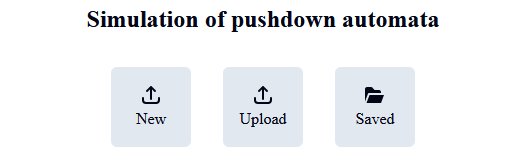
\includegraphics[width=0.8\textwidth]{Figures/PrntScrn_UI_MainMenu.png}
    \caption{Hlavní stránka}\label{fig:UIMainPage}
\end{figure}

\section{Stránka pro tvorbu zásobníkového automatu}\label{sec:PDABuilder}

Po kliknutí na tlačítko new v hlavní nabídce se otevře stránka pro tvorbu zásobníkového automatu. Tato stránka se skládá z několika formulářů a HTML input prvků. 

Jako první je textové pole pro specifikaci názvu automatu. Tento název se pak zobrazuje ve výpisu automatů z úložiště. Dále následuje formulář pro přidávání stavů. Stavy se přidávají po jednom a jejich délka není omezená.D8le následují formuláře pro definování vstupní a zásobníkové abecedy. Symboly se opět přidávají po jednom a jejich délka je omezena na jeden znak. Vstupní pole pro název a formulář pro přidávaní stavů lze vidět na obrázku~\ref{fig:BuilderPart1} včetně chybové hlášky.

\begin{figure}[h]
    \centering
    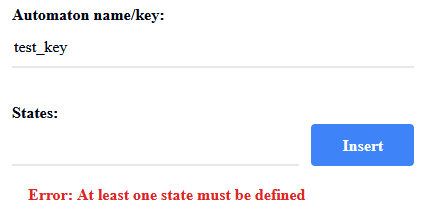
\includegraphics[width=0.5\textwidth]{Figures/PrntScrn_UI_BuilderPart1.png}
    \caption{Název a formulář pro přidávání stavů}\label{fig:BuilderPart1}
\end{figure}

Po těchto třech formulářích následují dva seznamy pro výběr počátečního stavu a počátečního zásobníkového symbolu. Po těchto dvou seznamech následuj část pro určení, zda zásobníkový automat bude přijímat prázdným zásobníkem nebo přijímací stavy. To závisí na tom, zda uživatel zaškrtne zaškrtávacího pole. Pokud zůstane nezaškrtnuté, musí uživatel vybrat alespoň jeden ze stavů níže jako přijímací. Seznam počátečních zásobníkových symbolů a zaškrtávací pole je na obrázku~\ref{fig:BuilderPart2}.

\begin{figure}[h]
    \centering
    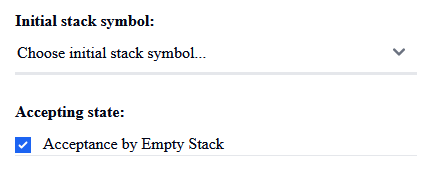
\includegraphics[width=0.5\textwidth]{Figures/PrntScrn_UI_BuilderPart2.png}
    \caption{Seznam počátečních zásobníkových symbolů a zaškrtávací pole pro určení typu zásobníkového automatu}\label{fig:BuilderPart2}
\end{figure}

Poslední část pak slouží k definování přechodů přechodové funkce. Její funkce již byla popsána v sekci~\ref{sec:PDABuilderImplementation}. Jak tato část vypadá lze vidět na obrázku~\ref{fig:FilledTransition}. Pak již následují jen tlačítka na navrácení na hlavní stránku a uložené zásobníkového automatu.

\section{Formulář pro nahrávání zásobníkových automatů}\label{sec:UploadForm}

Druhým tlačítkem v hlavní nabídce se uživatel dostane na stránku s formulářem, který slouží k nahrání zásobníkového automatu ze souboru. Formulář, obrázek~\ref{fig:UploadForm}, je složen ze dvou částí. První je textové pole pro pojmenování automatu. Toto pole se používá jako klíč pro úložiště a zároveň se zobrazuje v výpisu automatů. Pokud je klíč již použitý pro jiný automat, je při odeslání formuláře uživatel dotázán, zda chce automat s tímto klíčem přepsat. Druhé pole pak slouží pro nahrání souboru typu JSON, který obsahuje definici zásobníkového automatu. Při odeslání formuláře se nejprve ze souboru vytvoří instance třídy PushdownAutomata a následně se provede kontrola. Pokud automat nemohl být vytvořen kvůli neodpovídající struktuře nebo obsahuje chyby, je na to uživatel upozorněn společně s výpisem chyb, obrázek~\ref{fig:PDACheckErrors}.

\begin{figure}[h]
    \centering
    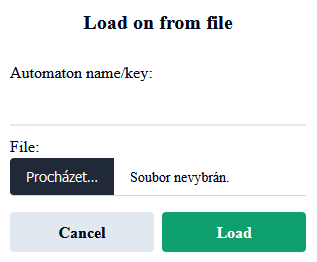
\includegraphics{Figures/PrntScrn_UI_Upload.png}
    \caption{Formulář pro nahrání zásobníkového automatu ze souboru}\label{fig:UploadForm}
\end{figure}

\section{Výpis úložiště}\label{sec:StoragePage}
\section{Simulátor}\label{sec:SimulatorPage}



\endinput